%---------------------------------------------------------------------
% Course 	: Introduction To web sciences
% Professor : Dr.Nelson
% Name   	: Babitha Bokka
% Assignment: 9
%---------------------------------------------------------------------
\documentclass[12pt]{article}
%--------------------------------------------------------------------
% packages required
%--------------------------------------------------------------------
\usepackage{graphicx}
\usepackage{listings}
\usepackage{hyperref}
\usepackage{caption}
\usepackage{color}
\usepackage{pdfpages}
\graphicspath{ {images/} }
%--------------------------------------------------------------------
% Start Margins
%--------------------------------------------------------------------
\addtolength{\oddsidemargin}{-.875in}
\addtolength{\evensidemargin}{-.875in}
\addtolength{\textwidth}{1.75in}
\addtolength{\topmargin}{-.885in}
\addtolength{\textheight}{1.95in}
%-------------------------------------------------------------------
% End Margins
%--------------------------------------------------------------------
\definecolor{codegreen}{rgb}{0,0.6,0}
\definecolor{codegray}{rgb}{0.5,0.5,0.5}
\definecolor{codepurple}{rgb}{0.58,0,0.82}
\definecolor{backcolour}{rgb}{0.95,0.95,0.92}
 
\lstdefinestyle{mystyle}{
    backgroundcolor=\color{backcolour},   
    commentstyle=\color{codegreen},
    keywordstyle=\color{magenta},
    numberstyle=\tiny\color{codegray},
    stringstyle=\color{codepurple},
    basicstyle=\footnotesize,
    breakatwhitespace=false,         
    breaklines=true,                 
    captionpos=b,                    
    keepspaces=true,                 
    numbers=left,                    
    numbersep=5pt,                  
    showspaces=false,                
    showstringspaces=false,
    showtabs=false,                  
    tabsize=2
}
 
\lstset{style=mystyle}

\begin{document}

%---------------------------------------------------------------------
%Making the title page
%---------------------------------------------------------------------
\begin{titlepage}
\title{INTRODUCTION TO WEB SCIENCES:\\*Assignment 9}
\author{Babitha Bokka}
\date{06 December 2014}
\maketitle
\end{titlepage}

%---------------------------------------------------------------------
%Table of contents
%---------------------------------------------------------------------
\tableofcontents
\newpage
%------------------------------------------------------------------
%Question 1
%------------------------------------------------------------------
\section{Question 1:}
\begin{verbatim}
Create a blog-term matrix.  Start by grabbing 100 blogs; include:

http://f-measure.blogspot.com/
http://ws-dl.blogspot.com/

and grab 98 more as per the method shown in class.

Use the blog title as the identifier for each blog (and row of the
matrix).  Use the terms from every item/title (RSS) or entry/title
(Atom) for the columns of the matrix.  The values are the frequency
of occurrence.  Essentially you are replicating the format of the
"blogdata.txt" file included with the PCI book code.  Limit the
number of terms to the most "popular" (i.e., frequent) 500 terms,
this is *after* the criteria on p. 32 (slide 7) has been satisfied.

Create a histogram of how many pages each blog has (e.g., 30
blogs with just one page, 27 with two pages, 29 with 3 pages and 
so on).
\end{verbatim}

%---------------------Approach----------------------------------
\subsection{Approach}
\begin{enumerate}
 \item In doing this assignment I took help from Mallika and Victor. They explained me about the packages to be installed and what to do? and what not to do?.
    \item To solve this questions I wrote shell script to grab the other 98 links.
    \item I wrote a short python script to append the ``feeds/posts/default?max-results=500''.
    \item And to get the top 500 words I modified feedparser.py.  
   
\end{enumerate}
   
\newpage
%-----------------------Source Code------------------------------
\subsection{Source Code}
\subsubsection{extractLinks.sh}
\lstinputlisting[breaklines=True]{../Q1/extractLinks.sh}
\subsubsection{makingAtoms.py}
\lstinputlisting[breaklines=True,language=Python]{../Q1/makingAtoms.py}
\newpage
\subsubsection{generatefeedvector.py}
\lstinputlisting[breaklines=True,language=Python]{../Q1/generatefeedvector.py}
\subsubsection{pagesEachBlog.py}
Could not finish  to generate the Histogram.
\lstinputlisting[breaklines=True,language=Python]{../Q1/pagesEachBlog.py}

%-----------------------Output Section---------------------------
\subsection{Output Files}
\begin{enumerate}
    \item The output for this question is a matix which is uploaded in Github blogdata.txt.
\end{enumerate}
\newpage
%------------------------------------------------------------------
%Question 2
%------------------------------------------------------------------
\section{Question 2:}
\begin{verbatim}
Create an ASCII and JPEG dendrogram that clusters (i.e., HAC)
the most similar blogs (see slides 12 & 13).  Include the JPEG in
your report and upload the ascii file to github (it will be too
unwieldy for inclusion in the report).
\end{verbatim}

%-----------------------Approach--------------------------------
\subsection{Approach}
\begin{enumerate}
    \item To answer this question I used clusters.py.
    \item Used the lines of code provided in the presentation.
	\item Python program generateAscii.py produces ASCII results which are piped to an output file ascii.txt.
	\item Also produces dendrogram blogclust.jpg.
\end{enumerate}

\newpage
%-----------------------Source Code-----------------------------
\subsection{Source Code}
\subsubsection{generateAscii.py}
\lstinputlisting[breaklines=True,language=Python]{../Q2/generateAscii.py}
\subsubsection{clusters.py}
This program is imported into question 2, 3 and 4.
\lstinputlisting[breaklines=True,language=Python]{../Q2/clusters.py}
\newpage

%-----------------------Output Section---------------------------
\subsection{Output Files}
\subsubsection{blogclust.jpg}
\begin{figure}[ht]
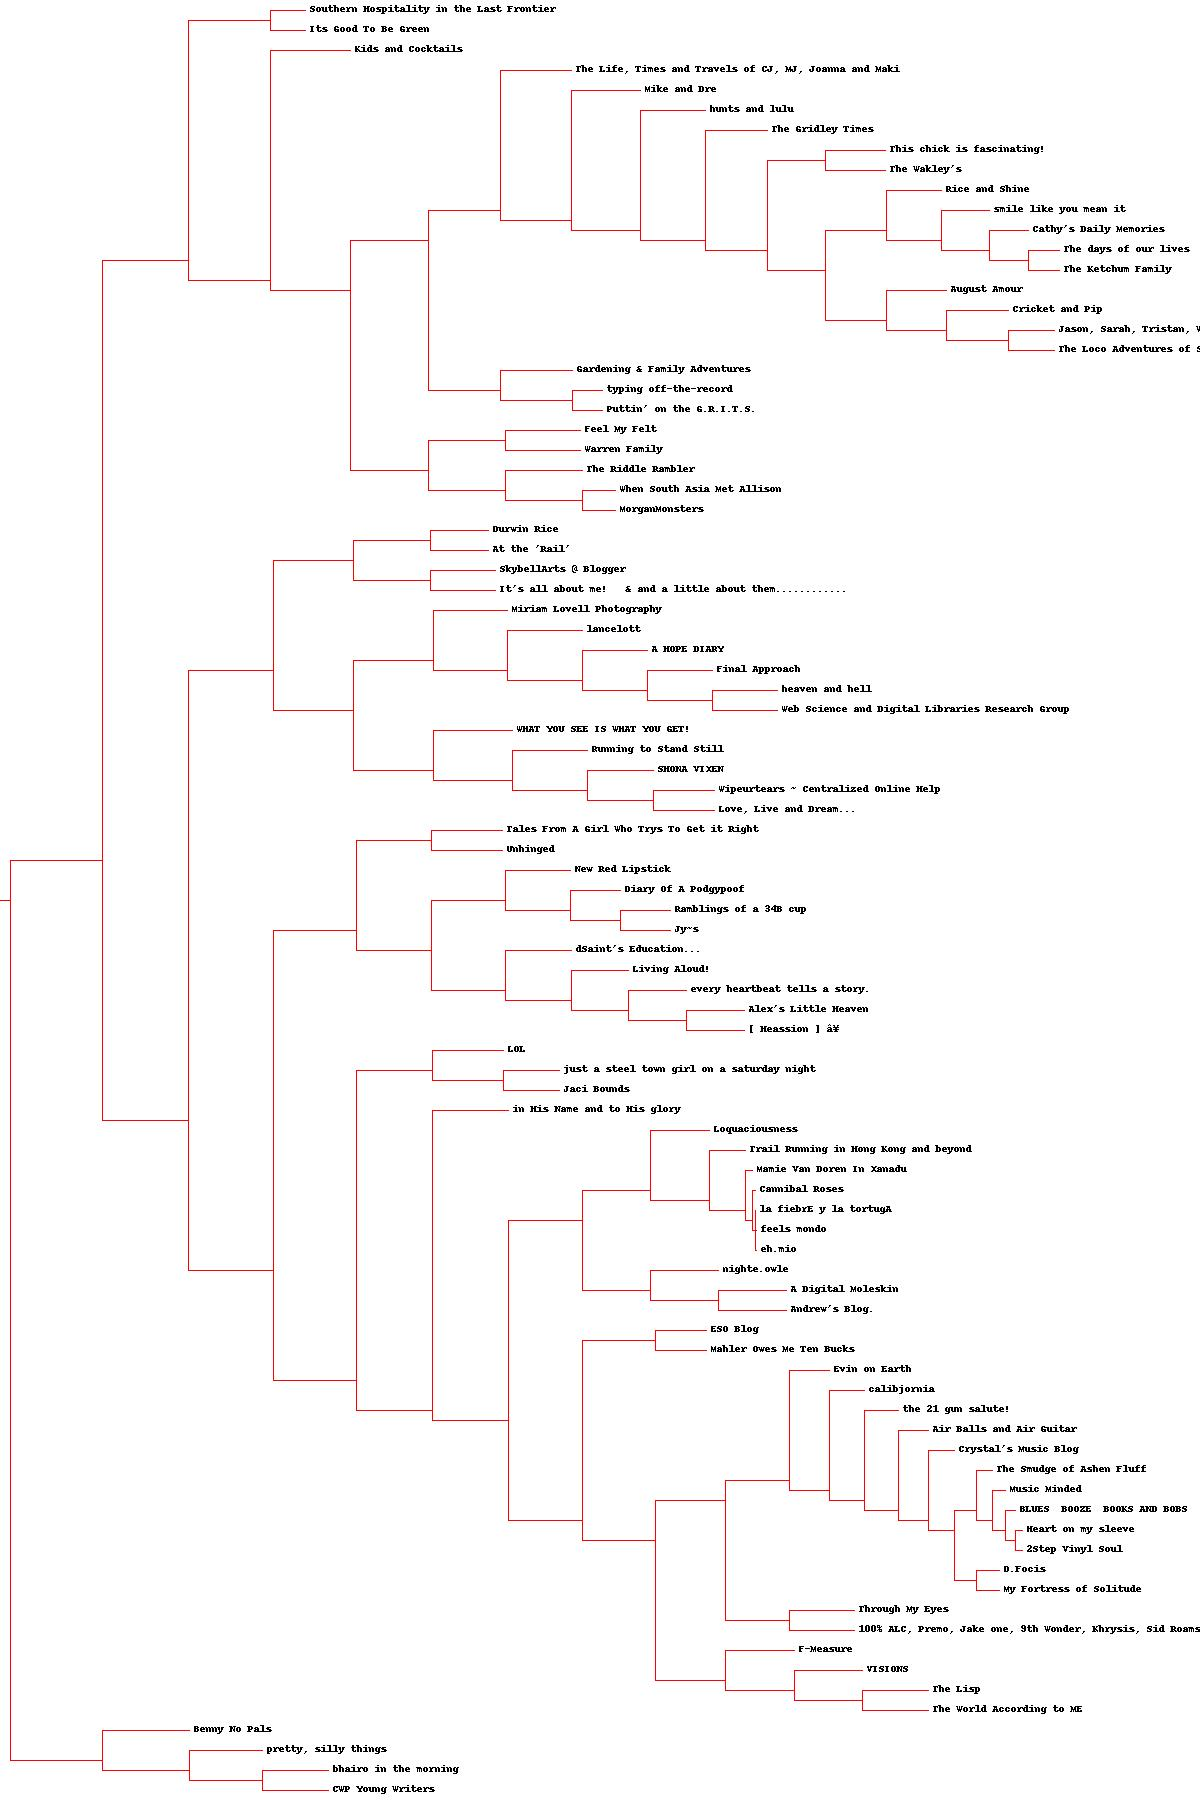
\includegraphics[scale=0.2]{../Q2/blogclust}
\centering
\caption{Dendrogram}
\label{fig:blogclust}
\end{figure}
\newpage


%------------------------------------------------------------------
%Question 
%------------------------------------------------------------------
\section{Question 3:}
\begin{verbatim}
 Cluster the blogs using K-Means, using k=5,10,20. (see slide 18).
How many interations were required for each value of k?
\end{verbatim}

%-----------------------Approach--------------------------------
\subsection{Approach}
\begin{enumerate}
    \item To solve this question I used lines of code provided in the presentation (calculateK-mean.py ) .
    \end{enumerate}

%-----------------------Source Code-----------------------------
\subsection{Source Code}
\subsubsection{calculateK-mean.py}
\lstinputlisting[breaklines=True,language=Python]{../Q3/calculateK-mean.py}
\newpage

%-----------------------Output Section---------------------------
\subsection{Output Files}
\subsubsection{output.png}
\begin{figure}[ht]
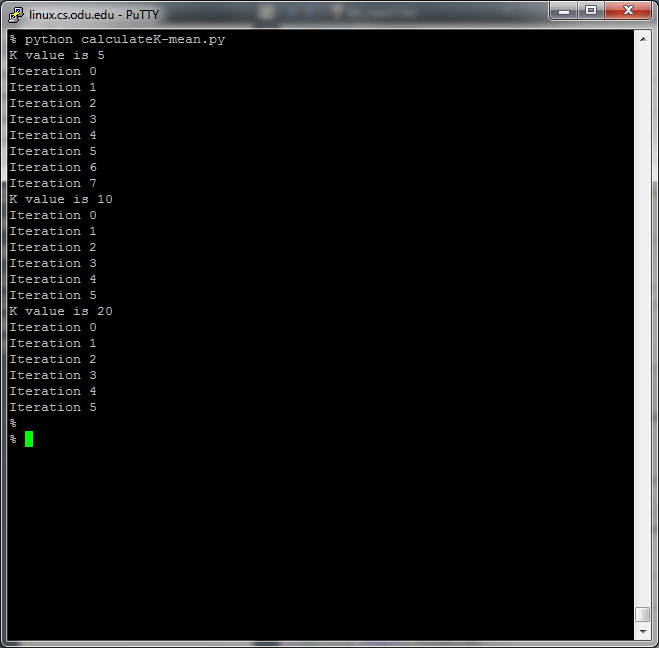
\includegraphics[scale=1.0]{../Q3/output}
\centering
\caption{Output of iterations for different k values }
\label{fig:blogclust}
\end{figure}
\newpage
%------------------------------------------------------------------
%Question 4
%------------------------------------------------------------------
\section{Question 4:}
\begin{verbatim}
 Use MDS to create a JPEG of the blogs similar to slide 29.  
How many iterations were required?
\end{verbatim}
%-----------------------Approach--------------------------------
\subsection{Approach}
\begin{enumerate}
    \item To solve this questions I used the few lines of code provided in the presentation (createMDS.py).
\end{enumerate}

%-----------------------Source Code-----------------------------
\subsection{Source Code}
\subsubsection{createMDS.py}
\lstinputlisting[breaklines=True,language=Python]{../Q4/createMDS.py}

%-----------------------Output Section---------------------------
\subsection{Output Files}
\begin{verbatim}
% python createMDS.py
4515.42807078
5524.56099361
% python createMDS.py
4299.13362421
5370.72157029
% python createMDS.py
4868.240652
7215.65051908
\end{verbatim}
\newpage

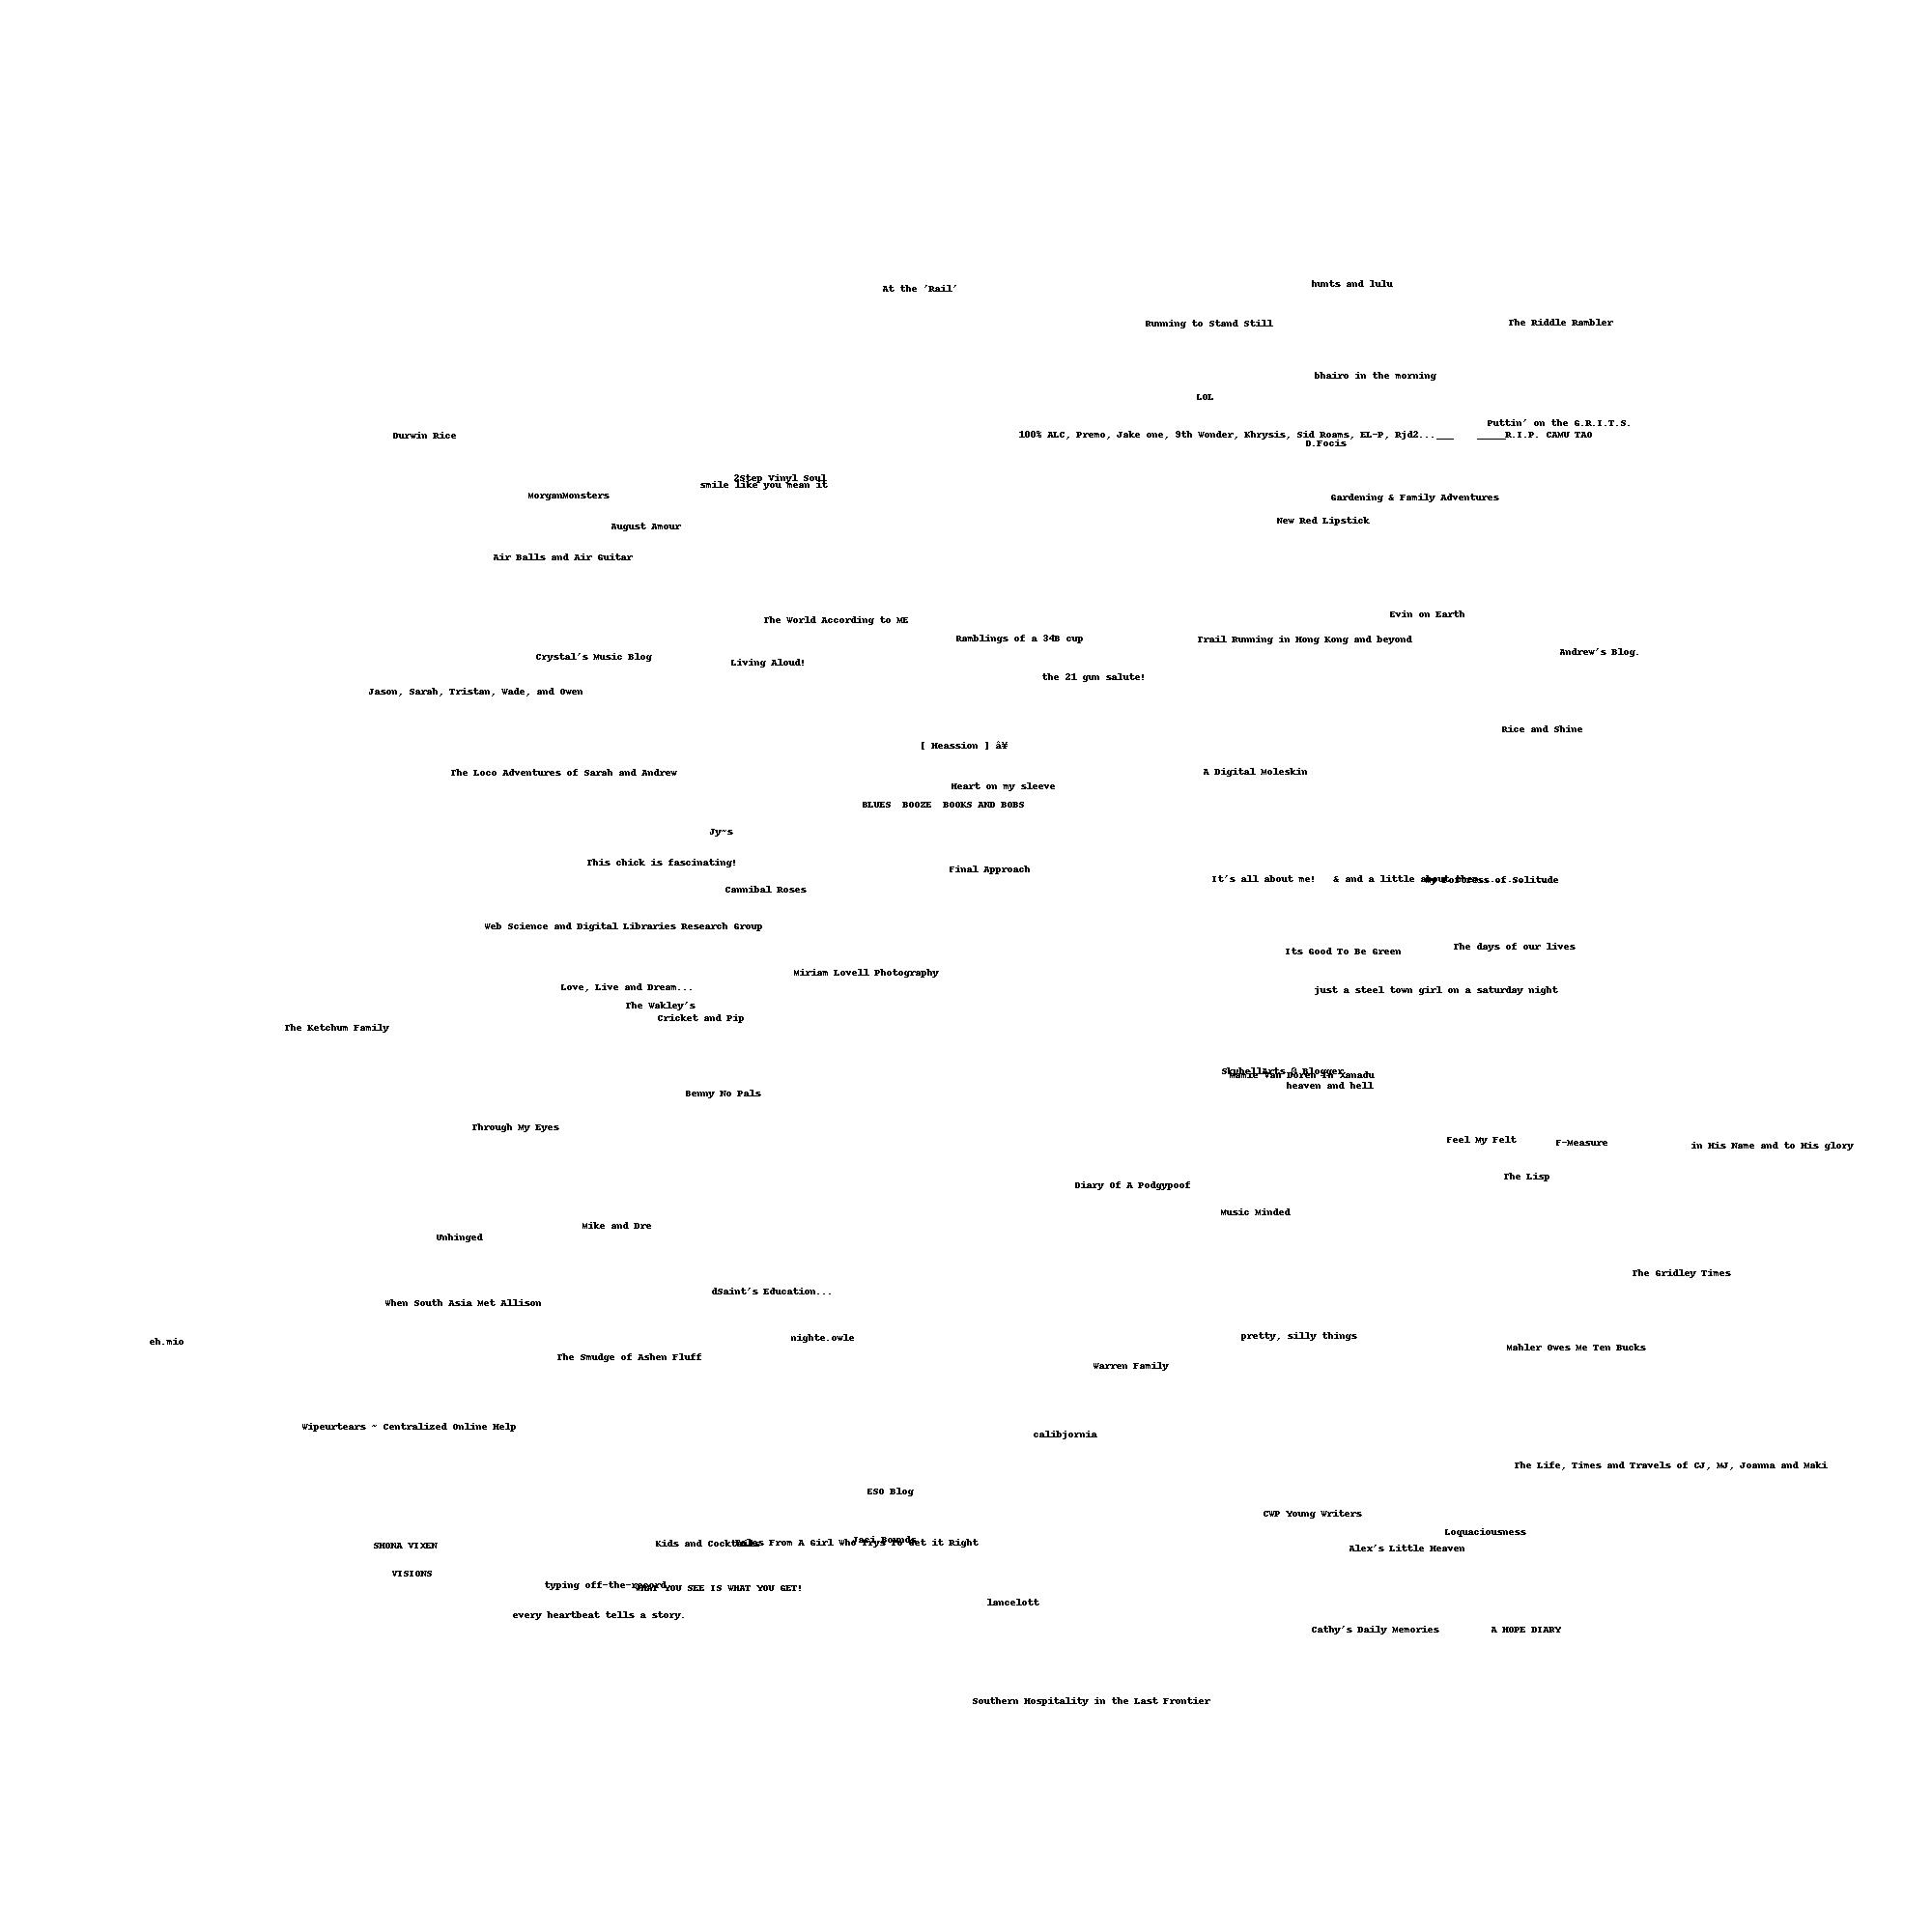
\includegraphics[scale=0.2]{../Q4/blogs2d}




\newpage

%------------------------------------------------------------------
%Bibilography
%------------------------------------------------------------------
\bibliographystyle{plain}
\bibliography{A9_report}
\cite{*}
\newpage
\end{document}